\documentclass[a4paper, 12pt]{article}

%---------Pacotes Usados-----------------+
\usepackage{amsmath,                    %|
            amssymb,                    %|
            amsfonts,                   %|
            latexsym,                   %|
            mathrsfs,                   %|
            amsthm,                     %|
            amstext,                    %|
            bezier,                     %|
            amscd}                      %|
                                        %|
\usepackage[top=2cm,                    %|
            bottom=2cm,                 %|
            left=2.5cm,                 %|
            right=2.5cm]                %|
            {geometry}                  %|
                                        %|
\usepackage{xcolor}                     %|
                                        %|
\usepackage{color}                      %|
\usepackage{hyperref}                   %|
\hypersetup{                            %|
    colorlinks=true,                    %|
    linktoc=all,                        %|
    linkcolor=black,                    %|
}                                       %|
                                        %|
                                        %|
\usepackage{soul}                       %|
                                        %|
\usepackage[utf8]{inputenc}             %|
                                        %|
\usepackage{indentfirst}                %|
                                        %|
\usepackage{graphicx}                   %|
                                        %|
\usepackage[portuguese]{babel}          %|
                                        %|
% Embelezando o cabeçalho e o rodapé    %|
\usepackage{fancyhdr}                   %|
\pagestyle{fancy}                       %|
\setlength{\headheight}{16pt}           %|
\addtolength{\topmargin}{-4pt}          %|
\fancyhf{}                              %|
\fancyhead[L]{\nouppercase{\leftmark}}  %|
\fancyhead[R]{\nouppercase{\rightmark}} %|
\fancyfoot[C]{\thepage}                 %|
\pagestyle{fancy}                       %|

% Configurando fbox para usar de moldura%|
% para imagens.
\setlength{\fboxrule}{1.2pt}

% Adicionando a capacidade de mostrar
% listas com duas colunas
\usepackage{multicol}
%----------------------------------------+


\begin{document}

%---------Infos MakeTitle----------------+
\title{                                 %|
\textbf{Anotações Definitivas}          %|
\break                                  %|
Aprendendo a usar \LaTeX\               %|
\vspace{5cm}                            %|
\begin{figure}[!htb]                    %|
\centering                              %|
\includegraphics[scale=.20]{latex_logo_folder.png}%|
\end{figure}                            %|
\vspace{4.5cm}                            %|
}                                       %|
\pagestyle{fancy}                       %|
                                        %|
\author{                                %|
    Lucas Gouveia Belon \\              %|
    lucasgouveiabelon@gmail.com         %|
}                                       %|
\date{\vspace{2.2cm}São Paulo\\2023}    %|
                                        %|
\maketitle                              %|
\newpage                                %|
%----------------------------------------+



%---------Sumário------------------------+
\tableofcontents                        %|
\thispagestyle{empty}                   %|
\newpage                                %|
%----------------------------------------+




%---------Estilos Próprios---------------+
\newcommand{\vimcommand}[1]{%
    \sethlcolor{black}%
    \textbf{\textcolor{white}{\hl{#1}}}%
}
\newcommand{\vimkeys}[1]{%
    \sethlcolor{black}%
    \textbf{\textcolor{red}{\hl{#1}}}%
}
%----------------------------------------+

% TODO: Encontrar uma imagem para adicionar na capa.

% TODO: Dar um jeito de diminuir o peso das imagens.
%\thispagestyle{empty}
%\setcounter{page}{-1}
%\thispagestyle{empty}

% Primeiro Capítulo
\section{Motivação}
Minha ideia original era aprender a utilizar o \LaTeX.
No entanto, é difícil aprender ambas as ferramentas.
Por conta disso, vou reescrever meu pequeno manual e fazer uma extensão com o que aprendi até então.
O uso de um editor específico com certeza simplifica muito as coisas, seja para edição de textos, seja para programação.
Porém, não é sempre que temos máquinas potentes o suficiente para isso.
O pacote de ferramentas que vem com o \LaTeX\ é gigantesco em variedade e em peso.

O pacote de ferramentas que acompanham qualquer outro software de edição de texto o são.
São alguns gigabytes de arquivos, muitas fontes, e diferentes compiladores.
Assustador, mas vamos com calma.
Este pequeno projeto é uma forma de eu me ambientar com o vimtex, e se ajudar alguém, é um ponto extra.

\subsection{Minha Motivação}
Quando comecei a faculdade havia a matéria de introdução à computação.
Nessa matéria sugeriu-se que se instalasse um Linux para fazer os exercícios e entender melhor sobre computação e afins.
De fato funcionou.
Comecei a aprender, e procurar, e aos poucos fui criando uma trilha de aprendizado.
Nessa trilha me encontrei com o terminal, ou prompt de comando, ou shell.
No Linux, é a forma mais eficiente de se executar uma tarefa.
Mesmo que muitas vezes não seja exatamente fácil, é possível salvar em um arquivo de script uma sequência de ações para que seja difícil uma única vez.
Isso me encantou.

Não bastasse isso, eu curso engenharia, e existem contas para se fazer,
procedimentos de cálculo, aproximações e avaliações que podem ser facilitadas com computadores.
Existem diferentes tipos de programas, e todos possuem essa natureza estranha, a existência dentro de computadores.

E para finalizar, todas as distribuições Linux conseguem rodar ao menos a linha de comando e um editor de textos.
E o VIM é um editor e tanto.

\subsection{Motivação Para Você}
Se você não dispõe de uma máquina potente, e precisa começar com programação, talvez seja um caminho muito mais difícil o que te espera.
Mas é no caminho mais difícil que temos a evolução mais acentuada.
Aprendi a programar em 2 linguagens de programação, das 3 que conheço, no celular.

Me bastou ter um aplicativo de emulação de terminal.
Tendo no terminal um editor e um compilador, aprendi C, uma das linguagens mais velhas que se tem por aí.
Além disso, fazer exercícios de programação mantém a mente afiada, e exige criatividade.
Com o básico bem estabelecido se chega realmente muito longe.

Se você possui um computador fraco, pode ser que instalar uma distribuição Linux alivie o peso.
Perde-se muitos aplicativos nativos do Windows, e muitas vezes suas tarefas dependem especificamente do Microsoft Office, ou do AutoCad, ou da suíte Adobe.
Mas também existe a possibilidade de se utilizar programas alternativos.
Existe também uma vantagem didática:
Não existe muita coisa no que prestar atenção para distrair se você está sempre utilizando o mínimo do mínimo.
E mesmo evoluindo na ferramenta, aprende-se compondo conhecimentos anteriores.
Dessa forma, quem aprende a mexer no vim acaba procurando pelos componentes de qualquer editor, para futura instalação e configuração.

Falando de ir além do básico, configurações em servidores são geralmente realizados sem interface gráfica.
Se trata de utilizar um computador distante, especializado em alguma tarefa.
E como eu disse antes, pode ser que pareça difícil, mas basta ser difícil uma única vez.

Uma única recomandação que me parece razoável, é a seguinte: Se você pretende escrever muito no computador, então vale a pena
aprender a digitar da forma correta.
Isso evita lesões por esforço repetitivo, aumenta a velocidade de digitação,
e, com isso, aproxima a velocidade de escrever com a velocidade de pensar.
Digitar enquanto se pensa torna o escrever uma expressão do pensar.

\subsection{Componentes}
O VIM possui pedaços.
E por ele começar tão simples que é uma ótima ferramenta para se evoluir.
Começamos com quase nada, e adicionamos camadas.

Outros programas de edição possuem os componentes que podem ser adicionados ao nosso editor favorito.
Outros componentes simplesmente não fazem sentido juntos dessa forma.
Pela versatilidade, e capacidade de se ter numa única ferramenta diversas configurações, decidi me dedicar a aprender.

\subsubsection{Editor de Texto}
O editor de texto é a parte núcleo, que quase todo servidor Linux possui.
Tem-se as funcionalidades básicas: Leitura; Escrita; Busca; Substituição.
E é aí que começa a ficar divertido.
Existe o que se chama de syntax highlighting, a capacidade de exibir o texto
com cores diferentes baseado na sintaxe, no sentido lógico usado.

Além disso, existem formas de se escrever, formas de se pensar, formas de se
mover o cursor pelo texto, que só fazem sentido dentro do vim.
Acontece que essa forma de se pensar é benéfica de tal forma que
editores de código especializados permitem integrar essa forma de se mover.

Temos também a gravação de macros, que são sequências de ações que podem ser tomadas e repetidas dentro de um texto.
Temos abreviações, que te impedem de escrever a mesma palavra errado e errado novamente, bastando configurar.
Também pode-se adicionar pequenos trechos de texto que são recorrentes no que se desenvolve.

Pode-se editar arquivos remotamente, pode-se utilizar abas,
e divisões de janela para visualizar mais de um arquivo ao mesmo tempo.
E pode-se invocar um terminal para continuar executando comandos do lado de fora, enquanto anota-se do lado de dentro.
É muita versatilidade.

\subsubsection{Configurações}
Arquivos de configuração fazem loucuras.
Existem templates de configuração, que nada mais são que pré configurações
que transformam e aproximam o vim de editores especializados para usos específicos.
Existem configurações que facilitam o uso, e outras que são impossíveis de se desacostumar.
Nos arquivos de configuração, tornam-se persistentes as alterações que também podem ser feitas com o editor aberto.

As configurações permitem alterar atalhos, e existe uma infinidade deles.
Permitem salvar macros, abreviações, mudar esquemas de cores, aparência e ergonomia do uso.
Basicamente, os arquivos de configuração fazem com que o editor fique com a sua cara.
No extremo, chega-se a um ponto em que alguém que também seja conhecido do vim não consiga usar o seu vim.
Nos arquivos de configuração também é onde se deixam plugins ativos.

\subsubsection{Plugins}
Para diversos usos, o vim é uma ferramenta tosca.
Não que seja impossível realizar qualquer tarefa com o básico do básico.
Mas se trata de uma ferramenta que começou com funcionalidades limitadas.
E programadores externos ao desenvolvimento da ferramenta possuem formas de
adicionar maneiras mais fáceis de se fazer uma tarefa.
Pensaram novas utilidades nunca antes pensadas, e extensões que se conectam com outros programas.

Talvez seja nos plugins que o vim deixa de ser uma ferramenta ruim para ser sincero.
Vê-se muitos vídeos, tantos vídeos, e blogs, e sites, sobre plugins que fazem isso e aquilo,
que faz parecer que a única função do vim é agregar todos os plugins num único ponto de encontro.

Mas não é bem assim. Existem muitas ferramentas já integradas, e hoje em dia não é tão ruim assim.
Vamos avançar a maior parte do livro sem eles.
Fazer dessa forma talvez mostre quais são os plugins que são essenciais pra você,
ao invés de instalar algo que faz o que já tem embutido, mas de um jeito mais bonitinho.

\subsection{Configurando Máquinas Remotas}
Servidores de dados, de e-mail, servidores web e o mundo na nuvem.
Todos são parte da mesma família de tecnologias.
Aprender uma ferramenta irá te ajudar a entender a próxima, e conseguir aprender mais rápido é motivador.

Essas máquinas remotas podem ser tão simples quanto um computador de 10 anos atrás, como podem ser super computadores, e ainda assim, são máquinas especializadas.
Não adianta querer jogar nessas máquinas.
Assim como não adianta querer fazer manobras de skate com uma tábua.
É parecido, mas se trata de outra coisa.

Se você chegou até aqui e aturou minha enrolação, então não tem motivo para não ir até o final.
Tentarei ser o mais prático possível.
Planejo fazer de tal forma que você possa abandonar o livro pela metade e se virar muito bem.
Mas muitas funcionalidades interessantes demoraram para serem colhidas e entendidas por esse cérebro
de geleia que está escrevendo. Então, vamos lá.

\newpage


% Segundo Capítulo
\chapter{Introdução}
Quando se trata de aprender a utilizar as funcionalidades avançadas de um editor de texto muito
antigo é preciso avançar um pequeno trecho por vez.
Para tecnologias antigas, existe na internet livremente todo tipo de dica,
todo tipo de vídeo, e até mesmo todo tipo de texto em pdf.
Mas um dos trabalhos deste documento é organizar para tornar mais orgânica a absorção.

O vim possui um tutorial, acessível pela linha de comando.
Basta escrever no seu prompt \vimcommand{\$ vimtutor} que o tutorial começa.
Assim como quase tudo na vida, você primeiro lê, depois tenta tomar alguma ação.
Pretendo seguir mais ou menos a mesma ordem do tutorial, mas com mais explicações.
Em alguns trechos teremos apenas a explicação e experimentar fica com você.

Para rodar o vimtutor, é preciso a versão do vim completa.
Portanto, o primeiro passo é instalar usando seu gerenciador de pacotes,
ou pesquisando na internet a forma de instalação para o seu sistema operacional.

\insertfigure{scale=0.90}{introducao/vimtutor_enter_screen.jpg}{O vimtutor é um bom ponto de partida.}

Uma espécie de piada que aparece em certos meios é sobre não se saber sair do vim.
Podemos começar por aí.
Podemos iniciar o vim com ou sem um nome de arquivo especificado.
Digamos que entramos sem especificar usando o comando \vimcommand{\$ vi}.
Assim que se abre o vim entra-se no modo \emph{normal}.
Através de teclas de atalho podemos entrar em outros modos.
Existem poucas formas de intercambiar entre modos, sendo geralmente mais simples voltar
para o modo normal antes de seguir para um outro.
Para voltar para o modo normal, pressione \vimcommand{esc} repetidamente,
ou mesmo a combinação \vimcommand{Ctrl-C} para desativar o modo atual.
Se você não fez nenhuma alteração no texto que está na tela
basta apertar \vimcommand{:} para entrar no modo \emph{ex}.
O modo ex serve para inserção de comandos.
Inseriremos o comando \vimcommand{:quit}.

\insertfigure{scale=0.9}{introducao/comando_quit.jpg}{Podemos sair do vim se quisermos.}

É parte da cultura Unix criar comandos como abreviações de nomes maiores,
como cat que abrevia con\textbf{cat}enate.
Você pode sair usando apenas \vimcommand{:q}.

Novamente com o vim aberto, pode-se escolher salvar o arquivo, definindo o nome, com \vimcommand{:write [nome do arquivo]}.
Atenção. Os comandos diferenciam minúsculas de maiúsculas.
Caso você esteja no modo normal, pode apertar \vimcommand{ZZ} para salvar e sair. Um atalho para \vimcommand{:wq}.

\section{Um pouco de qualidade de vida}
O vim cru não é exatamente muito legal.
Mas podemos melhorar usando umas poucas configurações logo de cara.
A primeira é quebrar o modo de compatibilidade com o antigo VI, usando o comando \vimcommand{:set nocompatible},
ou de forma abreviada \vimcommand{:set nocp}.
Dessa forma, você terá informações extras na última linha da janela, que farão falta se não estiverem habilitadas.

A próxima melhoria em qualidade de vida é adicionar números de linha com o comando \vimcommand{:set number}, ou \vimcommand{:set nu}.
Como dependemos da contagem de linhas para alguns movimentos e alguns comandos, tê-la à vista é interessante.

Outra configuração interessante é \vimcommand{:set ruler}.
Ela mostra no canto inferior direito informações sobre a posição do cursor.

Usando \vimcommand{:set laststatus=2} você irá criar uma barra permanente que indicará o nome do arquivo,
se ele está salvo, e as informações que ruler trouxe.

Usando \vimcommand{:set wildmenu}, você poderá ter seus comandos completados ao pressionar \vimkeys{$<$TAB$>$}.
Outra maneira de verificar quais as opções disponíveis é utilizar \vimkeys{$<$CTRL D$>$}.
Caso você esteja procurando entre muitas opções e não tem paciência para ficar pressionando tab,
\vimkeys{$<$CTRL D$>$} pode salvar tempo.

A última configuração serve para visualizarmos os comandos executados, úteis para macros.
Essa opção só está disponível no vim completo, mas como eu não sei qual vim você irá utilizar...
Usando \vimcommand{:set showcmd} aparecerão à direita as teclas pressionadas.
Será útil apenas mais adiante, mas ajuda na qualidade de vida.

Abra o vim com \vimcommand{\$ vi ~/.vimrc} e escreva cada um desses comandos.
Usar o vim padrão sem eles é terrível.

Os comandeos são:
\begin{itemize}
    \item set nocompatible
    \item set ruler
    \item set number
    \item set showcmd
    \item set wildmenu
    \item set laststatus=2
\end{itemize}

\insertfigure{scale=1.5}{introducao/vimrc_minimo.jpg}{Crie este arquivo pelo seu próprio bem.}

\section{Movimentação}
No modo normal fazemos as movimentações de cursor mais avançadas.
Dependendo da sua versão de vim, você pode usar as setas do teclado para se mover,
e pode realizar essa movimentação mesmo dentro do modo de inserção de texto.
Neste trecho do tutorial existe muito mais o que fazer do que mostrar,
então abra o seu vim e comece a testar.

Vamos ver o básico de movimentação:
\begin{itemize}
    \item \vimcommand{h} - Move para a esquerda.
    \item \vimcommand{j} - Move para baixo.
    \item \vimcommand{k} - Move para cima.
    \item \vimcommand{l} - Move para a direita.
\end{itemize}

\insertfigure{scale=0.8}{introducao/movim_minimo.jpg}{Movimentação básica.}


\subsection{Lógica Número-Ação-Movimento}
Em muitos casos podemos pedir que o vim interprete nossos comandos com um multiplicador.
Isso significa que, ao invés de pressionar \vimcommand{l} para andar para a direita 10 vezes,
podemos escrever \vimcommand{10l}, e a mágica acontece.
Essa lógica vai nos acompanhar, e inclusive vai ficar mais rebuscada à medida que começamos a misturar conhecimentos.
Futuramente colocaremos a ação na brincadeira, completando assim o número-ação-movimento.

% -------Movimentação por palavras -----------------

Além de movimentação em relação aos caracteres, podemos nos movimentar em relação às palavras.
Isso significa que podemos usar o equivalente a CTRL-direita ou CTRL-esquerda que temos em editores como o MS Word.
Para pular palavras a frente temos duas opções.
Pressionar \vimcommand{w} pula para a primeira letra da próxima palavra.
Para pular para a última letra da palavra mais próxima, \vimcommand{e}.
Usar estes comandos com letras maiúsculas irá ignorar pontuações, assim, apenas considerando espaços vazios.
Geralmente existem diferenças maiores entre comandos de letras maiúsculas e minúsculas.

Para voltar, \vimcommand{b}, que pula para a primeira letra da palavra anterior.
Para pular para a última letra da palavra anterior, \vimcommand{ge}.
Mais tarde vamos aprender que a tecla \vimcommand{g} é uma tecla separada para comandos sem muita lógica associada.
Talvez seja isso mesmo, genérico, geral.

Por fim, para simplificar: \vimcommand{w} vai pra próxima word. \vimcommand{b} faz um "backword".
Sempre bom encontrar maneiras de lembrar das palavras chave, mnemônicos ajudam.

% -------Movimentação na linha  -----------------

Podemos pular também para o começo ou fim da linha de texto.
Para pular para o primeiro caractere da linha, pressionamos \vimcommand{0}.
Para o último caractere, \vimcommand{\$}.
Quando desenvolvendo programas, existe a necessidade de se pular para o primeiro caractere não nulo.
Para fazer essa ação, podemos usar o comando \vimcommand{\^}.

Já falamos de palavras, de caracteres, e fomos para começo e fim da linha.
Podemos fazer o cursor viajar até um certo caractere.
Para essa ação escrevemos \vimcommand{t\_}, que significa "até o caractere \_".
A mesma ação, mas para trás, é usar \vimcommand{f\_}.
E, novamente, para ficar mais fácil de lembrar, "unTil \_".
E para a ação reversa, "find \_".

O uso de T e F fica a seu cargo de compreender.
Afinal de contas, não é porque não ensinei que você não vai aprender.

% -------Movimentação entre parênteses -----------------

Novamente, existe a funcionalidade de pular entre uma ponta ou outra de um pedaço de
texto que esteja dentro de parênteses, chaves ou colchetes.
Quando se está programando, isso faz muito sentido, já que existem grandes trechos de
códigos que podem estar enclausurados nestes caracteres.
A ação é \vimcommand{\%}.

% -------Movimentação entre parágrafos -----------------

Voltando ao texto normal, podemos pular parágrafos.
Estamos ficando bons em pular grandes trechos.
Para pular, \vimcommand{\{} e \vimcommand{\}}. Experimente.

% -------Movimentação pelo histórico de saltos -----------------

Sempre que fazemos um grande salto no vim deixamos um rastro na memória.
Podemos abusar disso para pular de forma eficiente.
Para voltar no histórico de pulos, \vimcommand{CTRL-O} para voltar.
Para avançar usamos \vimcommand{CTRL-I}.
Futuramente podemos verificar como pular entre palavras específicas.
Além disso, podemos pular entre palavras que não estão no mesmo arquivo aberto.

% -------Movimentação para começo/fim do arquivo -----------------
Para finalizar.
Podemos fazer mais dois tipos de salto, um para as pontas do arquivo, outro para um ponto qualquer.
O primeiro é pular para o começo do arquivo.
Usamos \vimcommand{gg}.
Para pular para o fim do arquivo, \vimcommand{G}.
E para pular para uma linha específica do arquivo, escrevemos \vimcommand{:n\'{u}mero}.

% -------Resumo dos comandos de movimentação de caracteres -----------------
Resumo:
\begin{itemize}
    \item Movimentação por caracteres:

        \subitem \vimcommand{h} - Esquerda.
        \subitem \vimcommand{j} - Baixo.
        \subitem \vimcommand{k} - Cima.
        \subitem \vimcommand{l} - Direita.

    \item Movimentação por palavras:

        \subitem \vimcommand{w}  - Avança para o começo da próxima palavra.
        \subitem \vimcommand{b}  - Retrocede para o começo da palavra atual.
        \subitem \vimcommand{e} - Avança para o fim da próxima palavra.
        \subitem \vimcommand{ge} - Retrocede para o fim da palavra atual.\\
        Obs: O uso de \vimcommand{W, B, E, gE} ignora pontuação levando em consideração apenas espaços em branco.

    \item Movimentação na linha:

        \subitem \vimcommand{0} - Começo absoluto da linha
        \subitem \vimcommand{\$} - Fim absoluto da linha
        \subitem \vimcommand{\^} - Começo não nulo da linha
        \subitem \vimcommand{t} - Avanço até certo caractere
        \subitem \vimcommand{f} - Retrocesso até certo caractere

    \item Movimentação entre parênteses, colchetes e chaves:

        \subitem \vimcommand{\%} - Pular entre começo e fim, priorizando o começo.

    \item Movimentação entre parágrafos:

        \subitem \vimcommand{\}} - Avança para o fim do parágrafo atual.
        \subitem \vimcommand{\{} - Retrocede para o começo do parágrafo anterior.

    \item Movimentação pelo histórico de saltos:

        \subitem \vimcommand{CTRL-I} - Avança para a posição no histórico de saltos.
        \subitem \vimcommand{CTRL-O} - Retrocede para a posição no histórico de saltos.

    \item Movimentação para primeira/última/alguma linha do arquivo:

        \subitem \vimcommand{G} - Avança para o fim do arquivo.
        \subitem \vimcommand{gg} - Retrocede para o começo do arquivo.
        \subitem \vimcommand{:12} - Salto para linha 12 do arquivo.

\end{itemize}
    
\subsection{Focando no Cursor}
Para lembrar, até agora estamos falando de funcionalidades que são factíveis no modo normal.

Agora que sabemos mudar a posição do cursor, vamos focar em um detalhe que ajuda na visualização.
Às vezes estamos escrevendo da direita pra esquerda, no sentido natural das coisas.
E naturalmente o cursor vai descendo.
Mas podemos mudar isso.

Para fazer com que o cursor fique focado focado ao centro da tela \vimcommand{zz}.
Importante. Não é a mesma coisa que \vimcommand{ZZ}, que salva e sai do programa.

Para fazer com que o cursor fique focado na parte do topo da tela, \vimcommand{zt}.
Para que fique na parte debaixo da tela, \vimcommand{zb}.

% -------Resumo Focando no Cursor -----------------
Resumo:
\begin{itemize}
    \item \vimcommand{zz} - Move a tela fazendo com que o cursor centralize.
    \item \vimcommand{zt} - Move a tela fazendo com que o cursor se apresente no topo da tela.
    \item \vimcommand{zb} - Move a tela fazendo com que o cursor se apresente na parte baixa da tela.
\end{itemize}

\subsection{Movendo a Tela}
Podemos pular de outras formas. Pular por páginas.

Para descer a tela apenas uma linha, \vimcommand{CTRL-e}. Para subir \vimcommand{CTRL-y}.
Perceba que o comando para subir fica na mão esquerda, para descer, mão direita.

Podemos descer a tela meia página, podemos usar \vimcommand{CTRL-d} e \vimcommand{CTRL-u}.
Para facilitar a memória, "d" é para "down" e "u" é para "up".

Por fim, chega de meia página, vamos mexer uma página inteira.
Use \vimcommand{CTRL-f} e \vimcommand{CTRL-b} para descer e subir.
Último mnemônico: "f" é para "fall", cair.
"b" é para "bring up", trazer para cima.
Caso nenhum mnemônico tenha te servido,
na mão esquerda estão as teclas que fazem a tela descer,
enquanto na direita estão as que fazem a tela subir.

Com isso, fechamos as movimentações.
Dizem que as movimentações do vim são a habilidade de ouro que fazem com que quem edita e escreve textos evolua.

Esses pulos, saltos, avanços, voltas, fazem com que quem precisa, principalmente, editar, consiga ter uma eficiência invejável.
Além de que parece bruxaria.

% -------Resumo dos comandos que movem a tela -----------------
Resumo:
\begin{itemize}
    \item \vimcommand{CTRL-e} - Desce a tela uma linha. Se necessário, desce o cursor uma linha.
    \item \vimcommand{CTRL-y} - Sobe a tela uma linha. Se necessário, sobe o cursor uma linha.
    \item \vimcommand{CTRL-d} - Desce a tela meia página. Tenta manter o cursor na mesma posição relativa.
    \item \vimcommand{CTRL-u} - Sobe a tela meia página. Tenta manter o cursor na mesma posição relativa.
    \item \vimcommand{CTRL-f} - Desce a tela uma página. Tenta manter o cursor na mesma posição relativa.
    \item \vimcommand{CTRL-b} - Sobe a tela uma página. Tenta manter o cursor na mesma posição relativa.
\end{itemize}

\section{Editando Texto}

\subsection{Inserir}
Inserir é provavelmente a coisa que você mais irá querer fazer.
O modo de inserção se assemelha muito aos aplicativos de bloco de notas mais comuns.
Para podermos entrar, finalmente, no modo que nos permite escrever texto dentro de nossos
arquivos e documentos, existem três formas.

Podemos inserir imediatamente acima do cursor utilizando \vimcommand{i}.
Utilizar o comando \vimcommand{I} te jogará para o começo não nulo da linha antes,
e também te colocará em modo de inserção.
Imagine como uma abreviação para \vimcommand{\^}\vimcommand{i}.

Para inserir imediatamente a frente do cursor, utilizamos \vimcommand{a}.
O comando \vimcommand{A} irá te jogar para o fim da linha e então será iniciado o modo de inserção.
Neste caso, pense como uma abreviação para \vimcommand{\$a}

Não bastasse podermos inserir em pontos da linha atual, podemos criar uma nova linha abaixo e inserir com \vimcommand{o}.
Se quisermos criar uma nova linha acima utilizamos \vimcommand{O}.
Existem casos em que escrevemos linhas parecidas, em que muito da linha anterior pode ser aproveitado para a linha atual.
Nesses casos podemos, quando dentro do modo de inserção, utilizar \vimcommand{CTRL-y} para copiar o que estiver escrito
na linha acima. Para copiar conteúdo, mas da linha debaixo, usamos \vimcommand{CTRL-e}.

% -------Resumo dos comandos para entrar no modo de inserção -----------------
Resumo:
\begin{itemize}
    \item \vimcommand{i} - Inicia o modo de inserção logo acima do cursor.
    \item \vimcommand{I} - Inicia o modo de inserção no começo não nulo da linha.
    \item \vimcommand{a} - Inicia o modo de inserção a frente do cursor.
    \item \vimcommand{a} - Inicia o modo de inserção no fim da linha.
    \item \vimcommand{o} - Cria uma nova linha abaixo e inicia o modo de inserção.
    \item \vimcommand{O} - Cria uma nova linha acima e inicia o modo de inserção.
    \item \vimcommand{CTRL-y} - Copia conteúdo, caractere a caractere, da linha acima do cursor.
    \item \vimcommand{CTRL-e} - Copia conteúdo, caractere a caractere, da linha abaixo do cursor.
\end{itemize}

\subsection{Deletar, Copiar, Colar}
Além de inserir, que provavelmente é a funcionalidade mais básica de um editor de textos, precisamos saber como apagar coisas.
Algo que é importante de deixar claro é que, tudo o que apagamos dentro do vim acaba ficando salvo no clipboard.
Isso significa que, se apagarmos uma linha, podemos usar o comando de colar, que a linha apagada irá voltar ao seu lugar.
E também que, se apagarmos duas linhas com dois comandos diferentes, apenas a última vai ficar salva neste "slot" de memória.

Para deletar um único caractere, pressione \vimcommand{x}.
Funciona como o delete, apagando o que o cursor ilumina, sempre a frente da linha.
\vimcommand{X} irá apagar a letra anterior ao cursor, tendo o efeito do backspace, sempre regredindo a linha.

Estes comandos obedecem a já falada lógica Número-Ação-Movimento.
A tecla \vimcommand{d} irá apagar a partir dessa lógica.
Fica mais claro com exemplos: \vimcommand{dl} irá apagar um caractere para a direita.
\vimcommand{dj} irá apagar a linha atual e a debaixo.
\vimcommand{dd} simplesmente apaga a linha atual.
\vimcommand{d\$} irá apagar da posição atual até o fim da linha.
\vimcommand{D} faz o mesmo que \vimcommand{d\$}.
E podemos misturar com um número para repetir a mesma ação n vezes.

Todas as movimentações de cursor são candidatas à composição dessas combinações.
Deletar até o próximo sinal de +? \vimcommand{dt+} fará o serviço.
E assim em diante.

O mesmo é válido para o comando de cópia.
\vimcommand{y}, significa "yank", e não faz muito sentido para quem fala português.
Mas serve para copiar um certo pedaço de texto.
Não se esqueça da lógica Número-Ação-Movimento, também serve para este comando.
\vimcommand{yy} irá copiar a linha atual, e o comando \vimcommand{Y} tem o mesmo efeito de \vimcommand{yy}.

Por fim, para colar temos duas opções: Ou copiar imediatamente acima do cursor, ou um caractere atrás.
Isso faz diferença quando estamos copiando uma linha, e acabamos por copiar o caractere de nova linha.
\vimcommand{P} copia no espaço imediatamente anterior ao cursor. \vimcommand{p} em cima do cursor.
Caso ainda não tenha ficado claro, o comando para recortar é o mesmo de apagar.

Como pode ser que você queira apagar um trecho de texto para imediatamente inserir algo em seu lugar,
Pode-se usar o comando \vimcommand{c}, que possui funcionalidade semelhante ao \vimcommand{d},
no entanto, após ser executado, troca para o modo de inserção.
Todo o anterior é válido, \vimcommand{c\$}, \vimcommand{c0}, \vimcommand{cj}, \vimcommand{ck}, e assim em diante.

% -------Resumo Deletar, Copiar, Colar -----------------
Resumo:
\begin{itemize}
    \item \vimcommand{x} - Deleta o caractere sob o cursor.
    \item \vimcommand{X} - Deleta o caractere imediatamente anterior ao cursor.
    \item \vimcommand{dd} - Deleta a linha atual.
    \item \vimcommand{d\$} - Deleta do caractere atual ao fim da linha.
    \item \vimcommand{D} - Deleta do caractere atual ao fim da linha.
    \item \vimcommand{dt+} - Deleta do caractere atual até o caractere +.
    \item \vimcommand{yy} - Copia a linha atual.
    \item \vimcommand{y\$} - Copia do caractere atual até o fim da linha.
    \item \vimcommand{p} - Cola sob o cursor.
    \item \vimcommand{P} - Cola na posição imediatamente anterior ao cursor.
    \item \vimcommand{cc} - Deleta a linha atual e entra no modo de inserção.
    \item \vimcommand{c\$} - Deleta do caractere atual até o fim da linha e entra no modo de inserção.
    \item \vimcommand{ct+} - Deleta do caractere atual até o caractere + e entra em modo de inserção.
\end{itemize}


\subsection{Substituir}
Caso seus erros sejam pequenos, e você queira substituir apenas um caractere sem sair do modo normal,
o comando \vimcommand{r} irá te inserir no modo Replace durante uma única pressionada.
Este comando permite trocar o caractere que estiver debaixo do cursor.

Para trocar sequências de caracteres, e assim, se manter no modo Replace por mais tempo, utilize o comando \vimcommand{R}.
Dessa forma, será preciso pressionar \vimcommand{esc} ou \vimcommand{CTRL-c} para voltar ao modo normal.

% -------Resumo Copiar, Colar, Substituir -----------------
Resumo:
\begin{itemize}
    \item \vimcommand{x/X} - Deleta o caractere debaixo/antes do cursor.
    \item \vimcommand{d/D} - Deleta de acordo com movimento/até o fim da linha.
    \item \vimcommand{y/Y} - Copia de acordo com o movimento/a linha atual.
    \item \vimcommand{p/P} - Cola a partir do cursor/um caractere antes do cursor
    \item \vimcommand{c/C} - Deleta de acordo com movimento/até o fim da linha e entra em modo de inserção.
    \item \vimcommand{r/R} - Substitui um caractere/uma cadeia de caracteres.
\end{itemize}

\subsection{Inside, Around}
Existem sequências avançadas, que lidam com o que é chamado de "objeto texto".
Um objeto texto pode ser um caractere, uma palavra, uma sentença, um paragrafo ou um bloco.
Vamos usar o comando "delete" para nossos exemplos, mas a lógica e a mecânica se aplicam também
para \vimcommand{y} e \vimcommand{c}.

Para deletar "abacate", mas preservar as aspas, podemos usar \vimcommand{diw},
que significa \textit{delete inner word}. Deletar a palavra interior.
As aspas servem como elementos de delimitação, o mesmo ocorreria com (banana).
No caso de deletar "caju", inclusive as aspas, podemos usar \vimcommand{daw},
que significa \textit{delete around word}. Deletar ao redor da palavra

Caso tenhamos uma frase, que se finaliza no ponto final,
e seja nosso desejo apagá-la, usamos \vimcommand{dis}.
Essa ação irá apagar a frase até o ponto final.
Nota-se que é importante o espaço em branco após o ponto entre uma frase e outra.
Sem ele, o vim não identifica corretamente a frase/sentença.
Para apagar o espaço em branco inclusive, \vimcommand{das}. 

Para apagar todo um parágrafo podemos usar \vimcommand{dip},
para manter o espaço abaixo do parágrafo.
Se quisermos apagar o espaço inclusive \vimcommand{dap}.

Existem dois tipos de bloco que o vim identifica imediatamente.
O bloco delimitado por parênteses pode ser deletado por \vimcommand{dib} ou \vimcommand{dab}.
Para o bloco delimitado por chaves podemos usar \vimcommand{diB} ou \vimcommand{daB}.

E caso queiramos apagar algo entre aspas simples? Nesse caso fazemos o seguinte:
\vimcommand{di\'} ou \vimcommand{da\'}.
É um tanto intuitivo, mas estou praticamente escrevendo \textit{delete inside "}.
Essa lógica funciona para quaisquer outros delimitadores

% -------Resumo Sequências Avançadas -----------------
Resumo:
\begin{itemize}
    \item \vimcommand{diw} - Deleta uma palavra
    \item \vimcommand{daw} - Deleta uma palavra, e seus arredores.
    \item \vimcommand{dis} - Deleta uma sentença/frase.
    \item \vimcommand{das} - Deleta uma sentença/frase e seus arredores.
    \item \vimcommand{dap} - Deleta um parágrafo.
    \item \vimcommand{dib} - Deleta um bloco delimitado por parênteses.
    \item \vimcommand{dab} - Deleta um bloco delimitado por parênteses e seus arredores.
    \item \vimcommand{diB} - Deleta um bloco delimitado por chaves.
    \item \vimcommand{daB} - Deleta um bloco delimitado por chaves e seus arredores.
    \item \vimcommand{di''} - Deleta um bloco delimitado por aspas duplas.
    \item \vimcommand{da''} - Deleta um bloco delimitado por aspas duplas e seus arredores.
\end{itemize}

\section{Modo Visual}
O modo visual te permite realizar uma ação que poderia muito bem ser executada com o mouse.
Caso seu vim esteja configurado para habilitar o mouse, ao segurar e arrastar para selecionar o texto, ele automaticamente irá trocar para o modo visual.
Então, sem muito mistério, uma das funcionalidades do modo visual é a seleção de pedaços de texto. Mas não para por aí.

Existem muitas ações que podem ser tomadas a partir de um texto selecionado. Você pode \textbf{visualmente} selecionar um texto antes de apagar.
Pode copiar um trecho específico.
Pode combinar comandos para utilizar esse trecho selecionado como um output.
E pode definir um escopo em que se pode realizar buscas.

\subsection{Modo Visual Normal}
No modo visual normal, você pode realizar as operações já especificadas.
Esse modo seleciona caracteres.
Para entrar neste, basta pressionar \vimcommand{v}, minúsculo.
Mova o cursor e você verá a seleção se mover também.
E caso você precise selecionar com o cursor mudando para a outra ponta, use o comando \vimcommand{o}.

\insertfigure{scale=0.5}{introducao/modo_visual.jpg}{Modo visual em ação.}

\subsection{Modo Visual Linha}
Neste, a seleção muda de lógica.
É muito eficiente para a seleção de trechos maiores.
Parágrafos, trechos de centenas de linhas, basta selecionar e então realizar sua ação.

\insertfigure{scale=0.5}{introducao/modo_visual_linha.jpg}{Modo visual-linha em ação.}

Destrua, reconstrua, altere ou defina um escopo para aplicar suas mudanças.
Para entrar neste modo, \vimcommand{V}, maiúsculo.

\subsection{Modo Visual Bloco}
A última variação do modo visual seleciona baseado em colunas.
Seu foco é a alteração de texto tabelado.
Também é interessante para a seleção vertical no geral, como em blocos de código que estão indentados.

Tudo o mais também é válido, seja salvar, recortar, ou usar como escopo para ações.
Para entrar neste modo, \vimcommand{CTRL-v}.

\insertfigure{scale=0.5}{introducao/modo_visual_bloco.jpg}{Modo visual-bloco em ação.}

\section{Undo, Redo}
É óbvio que a capacidade de desfazer alterações estaria presente por aqui também.
Para desfazer... \vimcommand{u} quando estiver no modo normal.
Para refazer... \vimcommand{CTRL-r} no modo normal.

No entanto, existe um tópico avançado que eu, particularmente, ainda não explorei, que é a árvore de mudanças que o vim guarda.
É possível navegar por versões alternativas, que surgem a partir de diferentes undo\'s e redo\'s.
No entanto, nem tudo que se pode aprender eu posso ensinar.
Se parece mágica e brilha aos seus olhos, corra atrás.
Te mostrarei como navegar pelo manual mais tarde, e você poderá aprofundar qualquer tópico.

Se a sua curiosidade é tanta que você deseja parar imediatamente a leitura para buscar, procure por \textit{"undo tree"}.

\section{Comandos Miscelâneos}
Enquanto ainda estamos falando sobre editar o texto, vamos para algo que não se relaciona muito bem com outros tópicos.
Podemos alterar a indentação e alternar entre maiúsculas e minúsculas sem entrar no modo de inserção.
E também podemos juntar linhas que estão atualmente separadas.

Para alterar a indentação de uma linha, \vimcommand{$<$}.
Talvez seja necessário utilizar o mesmo comando duas vezes, ou apertar espaço logo após o comando.
Este faz a indentação recuar.
Para avançar \vimcommand{$>$}

Para alternar entre minúsculas e maiúsculas dentro do texto, posicione o cursor no alvo
e \vimcommand{\~}, famoso til. 

Para juntar linhas, do inglês, \textit{join}, \vimcommand{J} maiúsculo.
Não tem muito mais o que dizer, apenas o que se testar e experimentar.

O rei dos comandos miscelâneos com certeza é a tecla \vimcommand{g}.
Para começar, quando uma linha fica comprida demais, e acontece o que se chama de wrap,
a linha começa a ser representada por um cojunto de linhas.
Mas o instinto é ainda assim, descer uma coluna, e dá errado usando apenas j e k.
Com \vimcommand{gj} e \vimcommand{gk} você pode descer uma linha no layout da linha.
Em outras palavras, \vimcommand{gj} e \vimcommand{gk} ignoram a contagem de linhas.

Para ir para o último caractere, usando a mesma lógica, temos \vimcommand{g0} e v\vimcommand{g\$}.
Mas vamos avançando. Aprendemos que podemos mudar a capitalização das letras, ou seja,
deixar maiúscula ou minúscula, pressionando \vimcommand{~}.
Bom, este é um comando como \vimcommand{x}, que não segue a lógica número-ação-movimento.
Usando \vimcommand{gu} para tornar minúscula, e \vimcommand{gU} para tornar maiúscula,
obtém-se esse super-poder.

Mas se o que você estiver procurando seja inverter a capitalização, ao invés de
deixar num estado definido, então usando \vimcommand{g~} você irá obter este
efeito, podendo inverter a capitalização de uma palavra, uma linha ou um
arquivo inteiro.

Quando selecionamos um trecho de texto, assim como com movimentações, deixamos um histórico para trás.
Para reselecionar no modo visual um trecho \vimcommand{gv} é seu cara.
Não espere eu te dizer o que alguns comandos fazem. Teste eles um por um.

Existe um comando meio duvidoso, que certamente trata-se do vim dando o melhor
de si, para executar alguma tarefa. Com \vimcommand{gq} você formata o texto num formato
semelhante à prosa. Não é recomendável utilizar para programas.
Talvez mais importante é não usar \vimcommand{gQ}, pois você entrará no modo \emph{ex} e jamais conseguirá sair.

Você já aprendeu que \vimcommand{J} junta linhas.
No entanto, ele preserva um espaço para indicar que os blocos de texto eram provenientes de linhas distintas.
Por isso, para eliminar esse espaço, \vimcommand{gJ} existe.
Não me pergunte o que ele faz.

Para terminar a miríade de comandos miscelâneos,
temos um comando para aplicar a última substituição realizada no documento inteiro.
Estamos falando do \vimcommand{g\&}, mais um dos comandos que não são bem parte da família de ninguém.

\section{Marks}
Esse tópico se confunde com outro, referente ao modelo de memória que o vim usa para armazenar diferentes tipos de dados.
Sempre que você realiza um salto, você deixa um rastro.
Mas e se você quiser armazenar uma posição para onde você pode voltar?

Futuramente vamos poder explorar a edição de múltiplos arquivos.
Imagine o potencial de deixar uma pequena marca em uma parte específica de um arquivo,
então digitar uma sequência de teclas, e o editor simplesmente te deixar onde você pode continuar o trabalho.
São saltos avançados.

Para definir uma marca, utilize o comando \vimcommand{:ma [caractere]}, e uma marca será definida na posição do cursor.
Para ir até a marca existem duas maneiras.
A primeira é utilizando o caractere crase \vimcommand{\`}\vimcommand{a}.
A segunda é utilizando aspas simples. \vimcommand{'}\vimcommand{a}.

O vim define marcas para todo tipo de coisa, seja qual foi sua última alteração de texto,
qual foi a última vez que entrou no modo de edição,
e até mesmo qual foi o último trecho que foi selecionado dentro do modo visual.

Para verificar quais os marks definidos, use \vimcommand{:marks}. Perceba quais são os caracteres utilizados para armazená-los.

Como existem muitos detalhes, e não é tudo que é interessante, fica como atividade para o leitor explorar no manual mais tarde.
Mas para completar a explicação, existem marcas salvas nos caracteres a-z, 
que são salvas referentes ao arquivo atual, e marcas salvas nos caracteres A-Z,
que salvam também o nome e caminho do arquivo.
Alguns caracteres são de uso automático, então ele provavelmente será sobrescrito, mas para saber quais são, leia o manual.

\insertfigure{scale=0.8}{introducao/marks_exemplo.jpg}{Lista de marks.}

\newpage


% Terceiro Capítulo
\chapter{Recursos avançados}
A maior parte do básico está feito.  Você sabe escrever, sabe apagar, sabe
trocar palavras de lugar, copiando e colando.  Já aprendeu a pular dentro
de um arquivo, fazendo parecer bruxaria.  Mas até agora estamos no reino
iluminado, em que se um iniciante observar pode conseguir entender o que
está acontecendo.  Eu diria que a partir de agora vamos mexer com magia
negra, pois se faltar atenção, nada será absorvido.  Por isso, a partir
daqui, teste tudo e crie você mesmo experimentos.

Vamos começar falando sobre como procurar e substituir termos e palavras
chave num arquivo e como podemos substituir estes.  Na sequência veremos o
que são os registros e para onde vão os trechos que apagamos.

Na sequência começaremos a usar múltiplos arquivos e executar ações neles.
Iremos organizar janelas para obter uma boa visualização, além de montar e
manter um layout eficiente.

\section{Busca No Arquivo}
Buscar dentro do arquivo é relativamente simples.
Basta usar o comando \vimcommand{/} e pesquisar o que você deseja encontrar.
Se for encontrado o termo, seu cursor será jogado para cima dele.
Se você estiver usando o vim completo, ao habilitar a opção \vimcommand{:set hlsearch},
suas buscas serão destacadas do texto com uma cor de fundo diferente.
Para que o destaque desapareça, é preciso rodar um comando,
\vimcommand{:nohlsearch}, ou a versão reduzida \vimcommand{:noh}. 

Para avançar entre os termos encontrados na busca, use o comando \vimcommand{n} para avançar.
Para retroceder, buscando termos anteriores, use \vimcommand{N}.
Na régua inferior podem aparecer informações importantes do tipo, "Sua busca chegou ao fim do arquivo, recomeçando",
vale a pena ficar de olho.

\insertfigure{scale=0.70}{recursos_avancados/Busca_No_Arquivo.jpg}{Mecanismo de busca com HighlightSearch.}

Podemos realizar buscas no sentido inverso do arquivo com \vimcommand{?}, que terá os mesmos impactos que a busca normal.
Caso você queira buscar um termo que esteja sob o cursor, pode-se utilizar \vimcommand{\#},
que o mesmo efeito de se utilizar a busca com \vimcommand{/} ocorrerá. 
Para se buscar o termo sob o cursor, mas no sentido inverso, vale o comando \vimcommand{*}\ .

Se você realizou uma busca e deseja repetí-la, \vimcommand{//}, e o mesmo vale para \vimcommand{??}.

O mecanismo de busca funciona normalmente no vim tiny, mas sem esse destaque.
Isso pode tornar difícil realizar uma busca válida, já que você pode nãoperceber com antecedência
que está escrevendo errado no campo de busca.

\insertfigure{scale=0.70}{recursos_avancados/Busca_No_Arquivo_vimtiny.jpg}{No vimtiny temos a mesma potência, mas não a mesma elegância.}

Apesar de podermos pesquisar termos simples, podemos também utilizar expressões regulares para encontrar padrões que se casam com nossas especificações.
Este é um texto sobre vim, não sobre REGEX, então, se quiser, vá atrás por conta.

\section{Substituição No Arquivo}
Quando estamos programando temos o costume de usar vastamente palavras chave.
A repetição de palavras chave é muito grande, seja para nomear variáveis, seja para nomear funções,
ou mesmo uma informação escrita à força, ou \textit{hardcoded}.
Você pode realizar a substituição de diversas formas diferentes.
Como você já sabe realizar a busca, basta encontrar e substituir uma a uma.
Mas, se você deseja fazer de uma forma automática, que abrange de uma ocorrência, a múltiplas delas, então esse comando é pra você.

Para realizar a substituição de uma ocorrência, na linha atual, pode-se usar:\\
\vimcommand{:s/ocorr/subst}.

\begin{figure}
\begin{center}
	\fbox{
	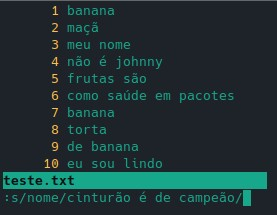
\includegraphics[scale=0.9]{recursos_avancados/Substituicao_simples.jpg}
	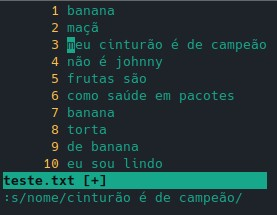
\includegraphics[scale=0.9]{recursos_avancados/Substituicao_simples_realizada.jpg}
	}
\caption{A substituição só ocorre na linha do cursor.}
\end{center}
\end{figure}

Perceba que você precisa estar com o cursor na linha alvo da substituição.
Se sua substituição tem como alvo todas as ocorrências de \textit{ocorr}, então,
com o cursor posicionado na linha alvo, \vimcommand{:s/ocorr/subst/g} dirá ao comando que
você deseja aplicar as substituições globalmente, alterando todas as ocorrências.

Para trabalhar com um escopo definido de linhas, existem duas formas: A primeira,
definir em quais linhas do arquivo a substituição ocorrerá.
Nesse formato fazemos \\
\vimcommand{:4,12s/ocorr/subst}
podendo aplicar na primeira ocorrência, ou em todas elas adicionando \vimcommand{g} ao final.
Neste exemplo, o escopo será da linha 4 à linha 12.

Uma outra forma de definir o escopo é selecionar com o modo visual o trecho
que sofrerá alteração.
Temos um pouco mais de flexibilidade neste caso, podendo selecionar pedaços de linha,
linhas inteiras,
blocos de texto\ldots\
E então, basta aplicar o comando.

Se quisermos que o escopo seja o arquivo inteiro, em todas as ocorrências, usamos \vimcommand{:\%s/ocorr/subst/g}.
O termo \% simboliza o próprio arquivo no vim.

\insertfigure{scale=1.20}{recursos_avancados/Substituicao_global.jpg}{A substituição global é muito poderosa, tome cuidado.}

\insertfigure{scale=1.20}{recursos_avancados/Substituicao_global_realizada.jpg}{Na barra inferior vemos quantas ocorrências foram afetadas.}

Para terminarmos sobre substuições, para que sejamos perguntados se queremos ou não substituir o termo de ocorrência:
\vimcommand{:\%s/ocorr/subst/gc}, o termo \vimcommand{c} adicionado é quem faz o serviço.

\section{Folds}
Existem casos em que você tem um parágrafo que deseja colapsar, ou seja, deixá-lo numa única linha para poder visualizar o restante.
Esta é mais uma funcionalidade que só existe no vim completo.
É útil para verificar a consistência do formato geral do texto, e para poder, por exemplo, verificar se todos os assuntos foram abrangidos.

Pessoalmente, acho raro utilizar, e difícil de configurar.
Mas caso você esbarre numa sequência de teclas estranhas, então melhor saber desfazer essas alterações.

A lista de teclas de ação são:
\begin{itemize}
    \item \vimcommand{zc} - Fechar uma dobra.
    \item \vimcommand{zo} - Abrir uma dobra.
    \item \vimcommand{zM} - Fechar todas as dobras.
    \item \vimcommand{zR} - Abrir todas as dobras.
    \item \vimcommand{za} - Abrir ou Fechar dobras.
\end{itemize}

Se você fechou uma dobra de texto, então poderá abrir.
Existem muitos métodos para identificar uma possível dobra que faça sentido.
Existem os métodos: \textit{indent}, \textit{diff}, \textit{syntax}, \textit{expr}, \textit{manual} e \textit{marker}.

Uma rápida explicação sobre o modo manual.
Utiliza-se \vimcommand{:set foldmethod=manual}, para ativar o método.
Seleciona-se uma quantidade de texto com o modo visual, e se usa o comando \vimcommand{:fold}.
Então você habilitou o trecho do texto a ser dobrável.
Eu considero uma forma trabalhosa, mas extremamente versátil.

\insertfigure{scale=0.70}{recursos_avancados/Fold_metodo_manual.jpg}{Folds são um assunto meio obscuro.}

\section{Registers}
Os registros do vim são os slots de memória de elementos salvos e deletados.
Nestes slots podem haver todos os tipos de informações.
Trata-se de conteúdo apagado, o clipboard do vim, nome do arquivo atual, do arquivo anteriormente aberto,
e macros, que são o conteúdo a seguir.

Para uma primeira experiência sobre os registros, vamos salvar um trecho de texto
em um slot específico: \vimcommand{''ax}, este comando irá ativar o registro \vimcommand{a}, e
o utilizará para armazenar o caractere que será apagado com o comando \vimcommand{x}.

Para colar um trecho de texto desse slot, o comando é parecido: \vimcommand{''aP}.
Perceba que escolhi utilizar o P maiúsculo, simplesmente para poder desfazer as alterações causadas pelo comando anterior.
Você pode visualizar quais registros estão sendo utilizados e seu conteúdo usando o comando \vimcommand{:registers}.
Se você vir caracteres esquisitos como \vimkeys{$<$80$>$} ou \vimkeys{\^}\vimkeys{M}, saiba que são caracteres especiais como 
enter, esc, ctrl-M, etc.
No meu vim em específico, como eu tenho algumas macros definidas, as ações de teclas especiais ficam salvas neste formato,
portanto, o vim possui um método próprio de armazenar caracteres de ação especiais.

\insertfigure{scale=0.75}{recursos_avancados/Registers.jpg}{Os registros armazenam todo tipo de informação.}

\section{Macros}
Macros fazem parte de um conjunto mágico de ferramentas que o vim possui.
Existem, para os editores de código, plugins para poder se aproveitar da movimentação que o vim oferece.
E de fato é muito bom poder se mover, saltar, salvar e fechar determinados arquivos.
Mas as macros são uma ferramenta muito específica, muito poderosa, que dificilmente pode ser imitada por um plugin.

Macros armazenam sequências de ações, sejam comandos, sejam inserção de texto, deleção ou substituição.
Literalmente qualquer coisa pode ser armazenada. Então, basta ativar a macro e sua ação será re-executada.

Vamos fazer um teste super simples.
A partir do modo normal pressione \vimcommand{q} e uma tecla para ser usada como registro.
No rodapé da janela você verá algo como \textit{''recording @a''}, que mostra que você está gravando
uma macro no registro "a".
Tecle novamente \vimcommand{q} para interromper a gravação.

Para testar, vamos fazer o seguinte:\vimcommand{qa0x\$xjq}.
Abrimos a gravação \vimcommand{q}, atribuímos o registro \vimcommand{a},
pedimos que retorne para o começo da linha \vimcommand{0}, que delete um caractere
\vimcommand{x}, que então pule para o fim da linha \vimcommand{\$}
e delete um caractere novamente \vimcommand{x}, e então descemos uma linha \vimcommand{j},
para enfim, encerrarmos a gravação \vimcommand{q}.

Difícil acompanhar apenas lendo, mas super simples de executar.
E talvez o mais importante, simples de replicar.
Para repetir esse conjunto de ações, selecione o número de repetições e use \vimcommand{$@$a}.
Essa macro deleta o primeiro e último caractere de uma linha e então pula para a linha seguinte.
Se você quisesse, por exemplo, deletar a primeira palavra de um conjunto de linhas, como faria?
Se a respostas for "à mão", então você está perdendo tempo e desperdiçando o potencial da ferramenta.

Para gravar macros, podemos utilizar dois tipos de operação.
Podemos sobrescrever um registro, que é o que fizemos no exemplo, mas podemos também adicionar novos comandos.
Basta pedir que seja gravada a macro num slot maiúsculo.
Ao usar \vimcommand{qAdiwjq}, estamos adicionando um "delete inner word" e um descer linha à macro salva no registro a.
Verifique com o comando \vimcommand{:registers} suas macros de teste.

Caso não tenha ficado claro, como as macros são armazenadas em um registro, podemos colá-las com \vimcommand{''aP}.
Isso será útil.
Caso pretenda alterar a macro, você pode colá-la, e alterá-la, e então voltar a salvar no slot.
Não é a maneira mais simples e elegante de se fazer isso, mas é uma forma.
O importante é perceber a complexidade e as aplicabilidades que macros possuem.

Quando falarmos de arquivos de configuração, o famoso vimrc, poderemos simplesmente colar nossa macro lá.
Dessa forma, teremos nossas macros sempre disponíveis, e poderemos criar macros cada vez mais elaboradas.
Pessoalmente possuo macros que servem de atalho para alguns comandos, outras para alteração de layout,
que é um tópico futuro, e uma com uma sequência de texto pré-definido.
O ponto negativo é gastar os slots, mas são muitos, e você pode simplesmente desativar essas configurações
futuramente, ou mesmo sobrescrever com um vazio.

\section{O Que É Um Buffer}
Quando programamos e precisamos reservar uma quantidade de memória do computador declaramos um buffer.
Basicamente, se trata de uma quantidade de memória reservada para operação.
Abrir arquivos é uma operação que requer um buffer, já que realizar alterações pequenas diretamente em arquivo
não é a melhor das ideias.
A estratégia é trazer para memória, alterar o trecho, e devolver as alterações para o armazenamento.

Quando você abre um arquivo, o vim cria um buffer.
Esse buffer representa seu arquivo.
Quando você salva, ele escreve as alterações no arquivo original.
E o mais importante, ninguém disse que não poderiam haver mais de um buffer.
Ou seja, vamos começar a abrir e editar mais de um arquivo por vez!

\section{Operando Com Múltiplos Arquivos}
Quando iniciamos o vim, podemos abrí-lo com um arquivo, como em \vimcommand{\$vim arquivo01.txt}.
Mas nada nos impede de abrir múltiplos, como em \vimcommand{\$vim arquivo01.txt arquivo02.txt}.
Quando abrimos dessa forma, imediatamente nos deparamos com o arquivo01.txt, mostrado em tela cheia,
sem indicações de que de fato abrimos o tal arquivo02.txt.
Para listar a pilha do buffer, usamos o comando \vimcommand{:ls}.
Perceba que eu disse pilha do buffer, e não lista de arquivos.
Não necessariamente iremos abrir arquivos, logo logo abriremos uma instância de terminal, e uma janela de navegação.

\insertfigure{scale=0.95}{recursos_avancados/Badd_ls.jpg}{Podemos carregar diferentes arquivos ao mesmo tempo.}

Para adicionar um novo buffer, mesmo que vazio, basta escrever \newline
\vimcommand{:badd nome\_do\_arquivo}.
Também temos o formato \vimcommand{:edit nome\_do\_arquivo}.
Não é muito clara a diferença entre eles, então fica a seu critério consultar o manual: \vimcommand{:help edit} e \vimcommand{:help badd}.
E para deletar temos duas formas: A primeira é escrever \vimcommand{:bdelete nome\_do\_arquivo}, mas
é uma forma problemática, já que requer lembrar o nome do arquivo.
Eu recomendo utilizar \vimcommand{:ls} e em seguida, pela numeração do buffer escolher qual será deletado:
\vimcommand{:bd 3} por exemplo.

Para saber o significado de cada um dos símbolos que acompanham a numeração dos buffers, veja o manual.
Também haverá uma explicação sobre o manual mais ao final do documento.

Antes de podermos transitar, saiba que, por padrão, o vim não te deixa sair de um buffer com modificações feitas.
Ele pede que você salve as alterações.
Por enquanto, para poder transitar sem necessidade de salvar, utilize o comando \vimcommand{:set hidden} para
que seja ignorado o estado do arquivo.
Futuramente iremos adicionar esse comando em nosso arquivo de configuração.
\begin{figure}
\begin{center}
	\fbox{
	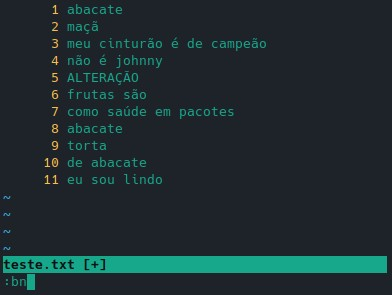
\includegraphics[height=5.4cm]{recursos_avancados/bn_setHidden.jpg}
	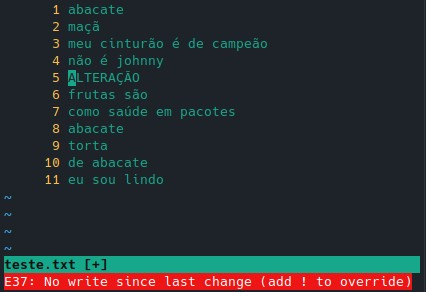
\includegraphics[height=5.4cm]{recursos_avancados/bn_error.jpg}
	}
\caption{Erro por não haver habilitado o modo hidden.}
\end{center}
\end{figure}

Agora que podemos adicionar e remover, vamos transitar entre os buffers, afinal de contas, é isso que interessa.
\vimcommand{:bnext} irá mudar para o próximo buffer da pilha.
\vimcommand{:bprevious} irá mudar para o buffer anterior da pilha.
\vimcommand{:bfirst} irá mudar para o primeiro buffer da pilha.
\vimcommand{:blast} irá mudar para o último buffer da pilha.
E pra finalizar, para pular para um buffer de número qualquer \vimcommand{:buffer \#}.

Todos esses comandos possuem formas simplificadas, exceto badd:
\begin{multicols}{2}
\begin{itemize}
    \item \vimcommand{:e} - Adicionar um buffer à pilha;
    \item \vimcommand{:badd} - Adicionar um buffer à pilha;
    \item \vimcommand{:bd} - Deletar um buffer da pilha;
    \item \vimcommand{:bn} - Ir ao próximo buffer;
    \item \vimcommand{:bp} - Ir ao buffer anterior;
    \item \vimcommand{:bf} - Ir ao primeiro buffer;
    \item \vimcommand{:bl} - Ir ao último buffer;
    \item \vimcommand{:b \#} - Ir ao buffer número \#;
\end{itemize}
\end{multicols}

Para abrir arquivos que estão inseridos dentro de pastas, ou que estão em pastas superiores,
depende-se de sintaxe de shell para caminhos relativos e absolutos, que eu suponho que você saiba.
Atenção, se você tentar abrir uma pasta acabará abrindo o navegador sem querer.
Teremos explicações sobre ele futuramente.

Existe um comando que abre todos os buffers numa janela, e isso entra no tópico a seguir.
Portanto, vou deixar aqui citado, e a explicação sobre como manipular fica no capítulo seguinte.
Para abrir todos os buffers na janela de uma só vez: \vimcommand{:ball}.

\insertfigure{scale=0.80}{recursos_avancados/ball_ls.jpg}{Vários buffers carregados.}

\vspace{1cm}
Apenas para citação: Existe um comando chamado bufdo, que executará uma ação em todos os buffers.
Com ele é possível rodar comandos, substituições e afins.
No entanto, a sintaxe é complexa, então vou deixar a cargo do leitor ir atrás de descobrir
se essas funcionalidades o são úteis.

\insertfigure{scale=0.80}{recursos_avancados/ball.jpg}{Usando \vimcommand{:ball} para abrir todos os buffers na janela.}

\section{MultiWindows}
Por hora conseguimos editar múltiplos arquivos.
A explicação sobre buffers serem como um espaço de memória, e sobre sua organização em pilhas
foi importante para sabermos como verificar quais arquivos estão carregados no vim.
Agora podemos dar passos significativos adiante.
Eu diria que esta é minha funcionalidade favorita desse editor.

Um detalhe importante que não citei antes por fazer diferença somente agora:
Existe uma diferença entre fechar com \vimcommand{:q} e deletar o buffer da pilha com \vimcommand{:bd}.
A diferença é que, com o comando \vimcommand{:q}, estamos fechando a janela em que o buffer se encontra,
mas se olharmos a lista de buffers com \vimcommand{:ls}, veremos que ele ainda está na pilha, e que,
portanto, pode ser novamente acessado.
Com \vimcommand{:bd} estamos descaregando da memória o arquivo, garantindo que as gravações foram ou feitas ou descartadas,
e liberando memória do editor.

\subsection{Invocando janelas}
Existem diversos comandos para abrir janelas.
Os dois primeiros, mais simples, são o \vimcommand{:new arquivo} que irá fazer com que a tela
se divida em duas horizontalmente, abrindo o novo buffer acima.
Já com o comando \vimcommand{:vertical new arquivo} o mesmo ocorre, mas verticalmente, e abrindo a nova janela à esquerda.

\insertfigure{scale=0.80}{recursos_avancados/split_new.jpg}{Abrindo uma nova janela.}

Outro conjunto, que faz mais jus ao nome das \textit{splitted Windows}, são os comandos \vimcommand{:split nome\_do\_arquivo} e 
\vimcommand{:vertical split nome\_do\_arquivo}.
Eles farão exatamente a mesma coisa que \vimcommand{:new} e \vimcommand{:vertical new}.

\insertfigure{scale=0.80}{recursos_avancados/vertical_split.jpg}{Abrindo uma janela vertical.}

Caso você já tenha carregado no editor a janela que deseja abrir, pode-se usar o comando
\vimcommand{:sbuffer}, ou \vimcommand{:vertical sbuffer}.
A vantagem de usar esse comando é a possibilidade de usar o comando \vimcommand{:ls}
para poder abrir a partir do número do buffer.

\insertfigure{scale=0.80}{recursos_avancados/vsbuffer.jpg}{Abrindo um buffer já carregado com vsbuffer.}
\insertfigure{scale=0.80}{recursos_avancados/vsbuffer_open.jpg}{Resultados semelhantes.}

Ficar limitado a sempre abrir à esquerda ou acima é complicado,
Mas temos a possibilidade de alterar qual será o local onde a nova janela irá nascer.

Como existem comandos para abrir verticalmente e horizontalmente, os comandos que definem
se a janela irá surgir acima/abaixo, na direita/esquerda, são colapsados.
E para complicar ainda mais, podemos por exemplo abrir logo à direita da janela atual, ou
abrir na extrema direita da tela.
E o mesmo para especificação vertical.

Para abrir algo logo abaixo ou à direita, use o comando \vimcommand{belowright}.
Perceba que, se usarmos o \vimcommand{split}, então ele irá mandar para baixo por conta do \vimcommand{below}.
Se usarmos o \vimcommand{vsplit}, irá abrir à direita, por conta do \vimcommand{right}.
Temos também os comandos \vimcommand{aboveleft},\vimcommand{botright}, e \vimcommand{topleft};
Com isso temos 8 combinações:
\vspace{1cm}

\begin{itemize}
    \item \vimcommand{:topleft split} - Abrir no topo da tela horizontalmente;
    \item \vimcommand{:botright split} - Abrir na base da tela horizontalmente;
    \item \vimcommand{:topleft vsplit} - Abrir no extremo esquerdo da tela verticalmente;
    \item \vimcommand{:botright vsplit} - Abrir no extremo direito da tela verticalmente;
    \item \vimcommand{:aboveleft split} - Abrir imediatamente acima da janela horizontalmente;
    \item \vimcommand{:belowright split} - Abrir imediatamente abaixo da janela horizontalmente;
    \item \vimcommand{:aboveleft vsplit} - Abrir imediatamente à esquerda da janela verticalmente;
    \item \vimcommand{:belowright vsplit} - Abrir imediatamente à direita da janela verticalmente;
\end{itemize}

\insertfigure{scale=0.80}{recursos_avancados/belowright_split.jpg}{Abrindo um buffer abaixo.}

Essas combinações realmente são muito ruins de se entender, principalmente por conta das indicações de direção
serem colapsadas em um único argumento.
Lembre-se, se o comando abre verticalmente, só importa esquerda e direita.
Se ele abre horizontalmente, só importa cima e baixo.

\insertfigure{scale=0.80}{recursos_avancados/aboveleft_vertical_sbuffer.jpg}{Efeito de aboveleft vertical sbuffer 4.}

\subsection{Alternando Entre Janelas E Movendo}
A forma mais simples de se mover entre janelas é usando \vimcommand{CTRL w CTRL w}, ou só \vimcommand{CTRL w w}.
Eu prefiro a primeira forma por já estar com o dedo no lugar.
Só com esse comando já podemos alternar legal entre as janelas. 
A lógica desse comando é alternar na ordem natural da escrita, que é, do topo para baixo, e da esquerda para a direita.

Mas claro que não vamos ficar limitados a esses movimentos simples.
O comando \vimcommand{CTRL w} habilita a movimentação.
Dessa forma, para ir para a janela da esquerda, basta usar \vimcommand{CTRL w l} para ir para a janela da direita.
Usando os comandos de movimentação \textit{hjkl} você se move para onde quiser.
Assim combinamos conhecimentos prévios:
\begin{itemize}
    \item \vimcommand{CTRL w h} - Troca para a janela da esquerda;
    \item \vimcommand{CTRL w l} - Troca para a janela da direita;
    \item \vimcommand{CTRL w j} - Troca para a janela debaixo;
    \item \vimcommand{CTRL w k} - Troca para a janela acima;
    \item \vimcommand{CTRL w t} - Troca para a janela superior (top);
    \item \vimcommand{CTRL w b} - Troca para a janela inferior (bottom);
\end{itemize}

\subsection{Redimensionando E Criando Um Layout}
Caso tenhamos aberto nossas janelas em uma disposição não muito agradável,
temos a opção de mover a janela para um dos cantos da tela.
Não temos como mover a janela com um controle muito bom, mas é melhor que nada.
Para mover a janela atual temos:

\begin{itemize}
    \item \vimcommand{CTRL w H} - Envia a janela atual para o canto esquerdo da tela;
    \item \vimcommand{CTRL w L} - Envia a janela atual para o canto direito da tela;
    \item \vimcommand{CTRL w J} - Envia a janela atual para o canto inferior da tela;
    \item \vimcommand{CTRL w K} - Envia a janela atual para o canto superior da tela;
    \item \vimcommand{CTRL w x} - Troca a janela atual de posição com seu vizinho mais próximo;
\end{itemize}

Podemos, por fim, redimensionar nossas janelas, seja com comandos, seja com atalhos.
Com comandos temos:

\begin{itemize}
    \item \vimcommand{CTRL w -} - Diminui verticalmente o tamanho da janela atual;
    \item \vimcommand{CTRL w +} - Aumenta verticalmente o tamanho da janela atual;
    \item \vimcommand{CTRL w $<$} - Diminui horizontalmente o tamanho da janela atual;
    \item \vimcommand{CTRL w $>$} - Aumenta horizontalmente o tamanho da janela atual;
    \item \vimcommand{CTRL w $|$ } - Aumenta verticalmente a janela atual ao máximo possível;
    \item \vimcommand{CTRL w \_ } - Aumenta horizontalmente a janela atual ao máximo possível (underscore);
\end{itemize}

No caso de redimensionar as janelas, é muito mais fácil editar algum atalho mais simples para a tarefa.
Eu particularmente deixo isso configurado, mas é bom saber qual o padrão, e saber mexer mesmo que não
seja na \textbf{sua} configuração.
É muito mais fácil alterar tamanho pedindo para redimensionar várias linhas ou colunas de uma vez.
Com atalhos conseguimos apenas uma linha ou uma coluna, ou os tamanhos máximos.
Os comandos abaixo estão escritos com o número 1, mas poderiam ser 5, 15, 55, o que o for razoável pra você.

Os comandos para alterar o tamanho das janelas são:
\begin{itemize}
    \item \vimcommand{:resize +1} - Aumenta verticalmente o tamanho da janela atual;
    \item \vimcommand{:resize -1} - Diminui verticalmente o tamanho da janela atual;
    \item \vimcommand{:vertical resize +1} - Aumenta horizontalmente o tamanho da janela atual;
    \item \vimcommand{:vertical resize -1} - Diminui horizontalmente o tamanho da janela atual;
    \item \vimcommand{:resize 35} - Torna o tamanho horizontal da janela como 35 linhas;
    \item \vimcommand{:vertical resize 35} - Torna o tamanho vertical da janela como 35 colunas;
\end{itemize}

Lembre-se, tamanho vertical refere-se à quantidade de colunas. Tamanho normal refere-se à quantidade de linhas.
Acabamos de encerrar o que há pra se saber sobre layout de janelas.

\insertfigure{scale=0.80}{recursos_avancados/resize.jpg}{Você pode manipular as dimensões das janelas à vontade.}

\section{MultiTabs}
Para quem entendeu a natureza de um buffer, e como as janelas servem apenas para mostrar os buffers
de maneira mais flexível, vai entender imediatamente as tabs (abas).
Assim como janelas organizam uma visualização de buffers, tabs organizam uma visualização de janelas.

Para criar uma nova aba, digamos uma aba com uma cópia do buffer atual, usamos o comando \vimcommand{:tabnew \%}.
Caso você tenha uma quantidade de abas abertas, e tiver o mouse ativado, você pode navegar clicando.
Também pode navegar por comando como \vimcommand{:tabNext}.

Caso você tenha uma quantidade de arquivos que deseja abrir, cada um em uma aba, na inicialização do vim,
pode-se usar \vimcommand{\$ vim -p arquivo1.txt arquivo2.py arquivo3.cpp}

Resumindo os comandos temos:
\begin{itemize}
    \item \vimcommand{:tabNew} - Cria uma nova aba;
    \item \vimcommand{:tabClose} - Fecha a aba atual. Não é o mesmo que deletar o buffer;
    \item \vimcommand{:tabprevious} - Move para a aba anterior;
    \item \vimcommand{gT} - Move para a aba anterior;
    \item \vimcommand{:tabmove -1} - Move a aba atual mais à esquerda na ordem das abas;
    \item \vimcommand{:tabnext} - Move para a próxima aba;
    \item \vimcommand{gt} - Move para a próxima aba;
    \item \vimcommand{:tabmove +1} - Move a aba atual mais à direita na ordem das abas;
    \item \vimcommand{:tabfirst} - Move para primeira aba.
    \item \vimcommand{:tablast} - Move para a última aba.
\end{itemize}

\insertfigure{scale=0.80}{recursos_avancados/tabnew.jpg}{Abas organizam layouts.}

Para mais informações, leia o manual com \vimcommand{:h tabpage}.
Usar abas é interessante para mover-se rapidamente entre arquivos que você sabe que utilizará.
Utilizar atalhos com estes comandos é uma grande vantagem.
Vreremos como configurar no vimrc.

\section{Save View}
Existem sessions e views como tentativas de salvar as configurações e layouts atuais.
Pessoalmente, nunca consegui utilizar direito as views, então vou deixar o manual aqui para você procurar:
\vimcommand{:help mkview}.
Acabamos de esgotar as funcionalidades do vim.tiny.
De agora em diante iremos utilizar somente prints do vim instalado completo.

\section{Netrw}
Caso você use o vim em sua versão completa, existe um navegador de arquivos embutido.
Num sistema com interface gráfica você certamente tem a capacidade de abrir um
explorador de arquivos, para navegar entre as diversas pastas que você não organiza.
Pois bem. O vim também tem algo parecido.

\insertfigure{scale=0.80}{recursos_avancados/netrwInicial.jpg}{Navegador de arquivos.}

O navegador NETRW nasceu como um plugin, mas atualmente está integrado ao vim.
E ainda bem que está.
Existem diversas formas de abrir o editor.
Pode-se usar o comando no terminal \vimcommand{\$ vim [pasta]} ou 
mesmo \vimcommand{\$ vim .}, e você estará no navegador de arquivos.
Mas e se você estiver dentro do vim, com seus arquivos já abertos?

Você pode usar o comando \vimcommand{:Explore} para carregar no buffer o explorador.
No entanto, agora que sabemos como funciona o sistema de janelas, podemos usar
\vimcommand{:topleft Vexplore} para assim adicionar uma janela para navegação.

A partir da janela de navegação podemos usar \vimkeys{$<$F1$>$} para abrir o menu
em uma janela horizontal. Lá você pode navegar até quickmap, onde estão as teclas de atalho mais básicas.
Pressionar enter em cima do nome de um arquivo fará com que este seja carregado na janela atual.
Usar \vimcommand{t} irá abrir o arquivo em uma nova aba.
Com \vimcommand{v} abriremos em uma aba vertical.
Ainda podemos deletar arquivos, criar pastas, e fazer o que comumente é possível num gerenciador de arquivos.

Existem funcionalidades diversas, como modo de exibição, tipo de acesso,
e outras coisas que eu não aprendi a usar.
O manual sobre o NETRW é extenso, e existem truques muito interessantes
que podem trazer um conforto sem igual à edição de textos por linha de comando,
seja código fonte para programadores, seja para a criação de manuais.

\section{Terminal}
Óbviamente, não poderia faltar.
Quando estamos programando, certamente iremos querer mexer aqui e acolá no terminal.
Vamos querer invocar o interpretador do código, compilar, ou mesmo rodar um comando simples.
A primeira opção é usar o que se chama de \emph{comando externo}.

Para rodar um comando na shell que você está usando usa-se \vimcommand{:!
[comando]}. Então se quisermos rodar o interpretador python para nosso
arquivo podemos fazer \vimcommand{:!python3 script.py} e tcharam, comando
executado. Esta é uma funcionalidade que o vim.tiny também possui.

Na outra opção, a lógica de nova janela segue sendo válida.
Para abrir uma janela de terminal na horizontal \vimcommand{:terminal}.
Para abrir na vertical \vimcommand{:vertical terminal}.

No caso do vim.tiny não temos uma janela de terminal aberta dentro do vim.
Ao invés disso, podemos apenas invocar um shell. Somos jogados em tela cheia para ele,
e quando pressionamos \vimcommand{\$ exit} voltamos ao vim padrão.
Para invocar o shell \vimcommand{:shell}.
Ele não possui a facilidade que o terminal possui, e é possível mimetizar esse comportamento
deixando o vim em background usando \vimkeys{$<$CTRL Z$>$}, para depois reativá-lo com
\vimcommand{\$ fg}.

\insertfigure{scale=0.80}{recursos_avancados/terminal.jpg}{Terminal aberto dentro do vim.}

Quando estamos utilizando terminais reais (no linux usamos o CTRL ALT F\#)
não temos a funcionalidade de histórico.
Abrindo o terminal a partir do vim, podemos torná-lo uma janela de texto qualquer,
nos permitindo navegar pelos comando já executados, e output's que ficaram para trás.
Para obter esse efeito \vimcommand{CTRL w N}, com N maiúsculo.

Página do manual: \vimcommand{:h terminal}.

\section{Save Session}
Caso você acabe com diversas abas, um layout elaborado de janelas com diversos arquivos,
enquanto trabalha num projeto relativamente grande, existe uma ferramenta muito útil para evitar
retrabalhos.

O vim te permite salvar o layout geral da seção.
No fundo, ele re-executa todos os comandos necessários para abrir as janelas,
na ordem e disposição que estavam da última vez.
Trata-se de um um arquivo em texto plano, ou seja, é possível abrí-lo com seu editor de textos favorito.

Acontece que, para conseguir esse armazenamento, acabamos com um arquivo relativamente grande,
mesmo para o layout mais simples.
Esse arquivo de layout, com extensão .vim, utiliza caminhos absolutos,
o que significa que se você mudá-lo de lugar, simplesmente seus arquivos não serão carregados.
No entanto, iremos ver uma função que é capaz de solucionar este problema.

O comando mágico para criar esse arquivo que salva o layout é \vimcommand{:mksession Session.vim}.
Para carregar o layout existem duas formas.
No momento de abrir o vim pode-se usar \vimcommand{\$ vim -S Session.vim}, ou dentro do próprio vim
podemos usar \vimcommand{:source Session.vim}.
O nome e a extensão não são realmente obrigatórios, mas manter um padrão é interessante.

Para encontrar os assuntos no manual, utilize o comando \vimcommand{:h session}.
Neste trecho de manual também é possível encontrar informações sobre views.

\section{Quickfix}
O quickfix é uma janela com itens selecionados que nos ajudam a nos localizar, a ler um pequeno trecho, e a nos locomover.
As janelas quickfix são uma variação das janelas preview.
De certa forma, elas nos permitem realizar busca e locomoção através de vários arquivos.
A grande vantagem é não precisar saber qual o arquivo, apenas qual o termo que queremos encontrar.

Se você compilar um programa usando os compiladores que o vim possui integração, ou mesmo se possui um servidor de linguagem,
um lsp, é possível que uma janela de quickfix seja acessível usando algo como \vimcommand{:LspDocumentDiagnostics}.

Como essa funcionalidade nasceu a partir de obter os erros que compiladores apontam, o comando base é \vimcommand{:c\#}, ou seja,
c alguma coisa.

Para, por exemplo, pesquisar sobre o termo \vimkeys{Hello} que pode estar em qualquer
arquivo do código fonte escrito em C, fazemos o seguinte: \vimcommand{:vimgrep ''Hello'' **.\{sh,py,c\}}.
O que fizemos foi procurar o termo "Hello" em qualquer subdiretório (**), em arquivos com um nome qualquer (*)
que terminem em ".c".
É razoável evitar buscas em diretorios muito profundos, já que o vim não consegue interromper a busca.
O padrão de busca por termo aceita REGEX, e a especificação por diretório aceita a sintaxe de comandos do shell.
A forma abreviada do comando \vimcommand{:vimgrep} é \vimcommand{:vim}.
Caso o programa "grep" esteja disponível em seu ambiente, \vimcommand{:grep} pode fazer o serviço.

\insertfigure{scale=0.80}{recursos_avancados/quickfixGenerate.jpg}{Gerando um quickfix.}

Com a busca executada e desde que algum termo tenha sido encontrado, acabamos gerando uma lista quickfix.
Para visualizar essa lista usamos \vimcommand{:copen}.
Se repousarmos nosso cursor em alguma linha da lista e pressionarmos enter,
seremos lançados para o arquivo, já com o cursor sobre o termo.

\insertfigure{scale=0.80}{recursos_avancados/quickfixLista.jpg}{Visualizando o quickfix.}

Digamos que não queremos ficar pulando de janela, apenas pular para o próximo termo encontrado na busca: \vimcommand{:cnext}.
Uma alternativa é usar apenas \vimcommand{:cn}. 
E é uma boa ideia atribuir um atalho para este comando.
Para pular para o termo anterior, \vimcommand{:cprevious}.
E por fim, para fechar a janela do quickfix, \vimcommand{:cclose}.

Para finalizar o uso básico, você pode tomar ações sobre os termos encontrados na lista com \vimcommand{:cdo}.
Funciona assim como podemos fazer com tabs ou buffers.

Para ler o manual: \vimcommand{:h preview}, \vimcommand{:h quickfix}, \vimcommand{:h vimgrep} e \vimcommand{:h grep}.
Esta é uma das funcionalidades que aprendi enquanto escrevia este documento.
Caso você se interesse apenas por escrever textos a lista quickfix pode não ser muito mágica.
Para quem programa, usando funções, repetindo termos em todos os lugares, em diversos arquivos,
é uma funcionalidade muito interessante.

A quickfix list é global para a sessão do vim, o que significa que ele irá substituir a janela que estiver aberta.
A location list é local à janela aberta, o que significa que você pode ter múltiplas location lists, mas apenas uma quickfix list.
Os comandos são semelhantes aos vistos anteriormente: \vimcommand{:lopen} \vimcommand{:lclose} \vimcommand{:lnext} \vimcommand{:lprevious}.

Para o manual: \vimcommand{:h lvimgrep} \vimcommand{:h lgrep} e \vimcommand{:h location}.

\section{Usando arquivos de tag}
O contexto da programação acaba gerando ferramentas interessantes para programadores.
Digamos que existe uma função a qual você ddseja inspecionar.
Certamente iria querer ver sua declaração, sua implementação, ou sua ordem de chamadas.
Arquivos tag criam um índice do qual o vim pode fazer uso para se locomover.
Existem plugins que gerenciam a criação e atualização das tags,
mas para um primeiro momento é mais interessante fazer as coisas manualmente.

Muitas vezes o programa que cria tags é instalado juntamente ao vim pelo gerenciador de pacotes.
Caso não esteja disponível, use seu gerenciador para instalar o ctags.
Para utilizar esses saltos é necessária a criacão de um  arquivo índice,
este terá como função especificar a estrutura de projeto,
e onde as palavras chave se encontram.

Para utilizar, vá até a raiz do seu projeto, e use o comando \vimcommand{\$ ctags -R *}.
Esse comando buscou todos os arquivos recursivamente em todos os subdiretórios.
O tal índice será salvo num arquivo em texto plano. Se quiser, inspecione-o.
Não se recomenda utilizar buscas recursivas em um diretório muito profundo.

Abra seu vim normalmente, de preferência em um arquivo de programção.
Em seguida, posicione o cursor em uma função que está sendo chamada,
para finalmente pressionar \vimcommand{CTRL ]}.
Supostamente você será jogado para a declaração da função.

Para fazer o caminho inverso, o comando \vimcommand{CTRL t}.

Digamos que você saiba o nome da função, mas não lembra em qual arquivo ela se encontra.
Você pode usar o comando \vimcommand{:tag funcao\_muito\_louca}.

Caso ocorram problemas com o comando \vimcommand{CTRL ]},
por ser o comando \vimkeys{Escape} do prompt de telnet,
você pode alterar a tecla remapeando.
Aprenderemos a remapear futuramente.

O programa ctags criou uma lista de tags.
Veja como elas são carregadas no vim com o comando \vimcommand{:tags}.
O sinal \vimkeys{$>$} indica qual a tag ativa.
Usar o comando \vimcommand{CTRL t} ou \vimcommand{:pop} irá usar essa posição.

Arquivos tag são realmente muito interessantes para programadores.
Existem alguns plugins que gerenciam os arquivos, sendo capazes de gerar e gerir,
à medida que arquivos são alterados e salvos no projeto.
Quando falarmos sobre plugins iremos procurar algum que faça essa função.

\newpage


% Quarto Capítulo
\section{Settings}
...
\subsection{Onde Estão Minhas Configurações}
...
\subsection{Abreviações}
...
\subsection{Salvando Macros}
...
\subsection{Olhando um arquivo vimrc pré-pronto}
...
\newpage
\section{Escolhendo e gerenciando Plugins}
...

\newpage
\section{Usando o Manual}
...

\newpage
\section{Usos diversos}
\subsection{PairProgramming com tmux}
\ldots
\subsection{Usando ssh-keys para editar arquivos remotos usando o meu vim}
\ldots
\subsection{Criando um layout semelhante à uma IDE (meu @i) com o vim padrão}
\ldots
\subsection{Usando ctags para saltos acrobáticos dentro de um projeto de programação}
\ldots

% TODO:Anotações finais: Adicionar qual página de manual cada uma das partes deve ler.
% Seria interessante também se eu mesmo pegar pra ler cada uma das páginas do manual,
% tanto pra aprender um pouco mais, quanto pra corrigir e adicionar novos usos
% que podem ser interessantes. Eita projetinho doido.
\end{document}
